\documentclass[tikz,border=12pt]{standalone}
\usepackage[utf8]{inputenc}\usepackage[T1]{fontenc}\usepackage{tikz}
\usetikzlibrary{arrows.meta,positioning,shadows.blur,shapes.geometric}
\definecolor{greenFill}{HTML}{E8F5E9}\definecolor{greenStroke}{HTML}{43A047}
\definecolor{coreFill}{HTML}{E1F5FE}\definecolor{coreStroke}{HTML}{0277BD}
\definecolor{memFill}{HTML}{FFF3E0}\definecolor{memStroke}{HTML}{EF8C00}
\definecolor{procFill}{HTML}{FFF9C4}\definecolor{procStroke}{HTML}{B38600}
\begin{document}
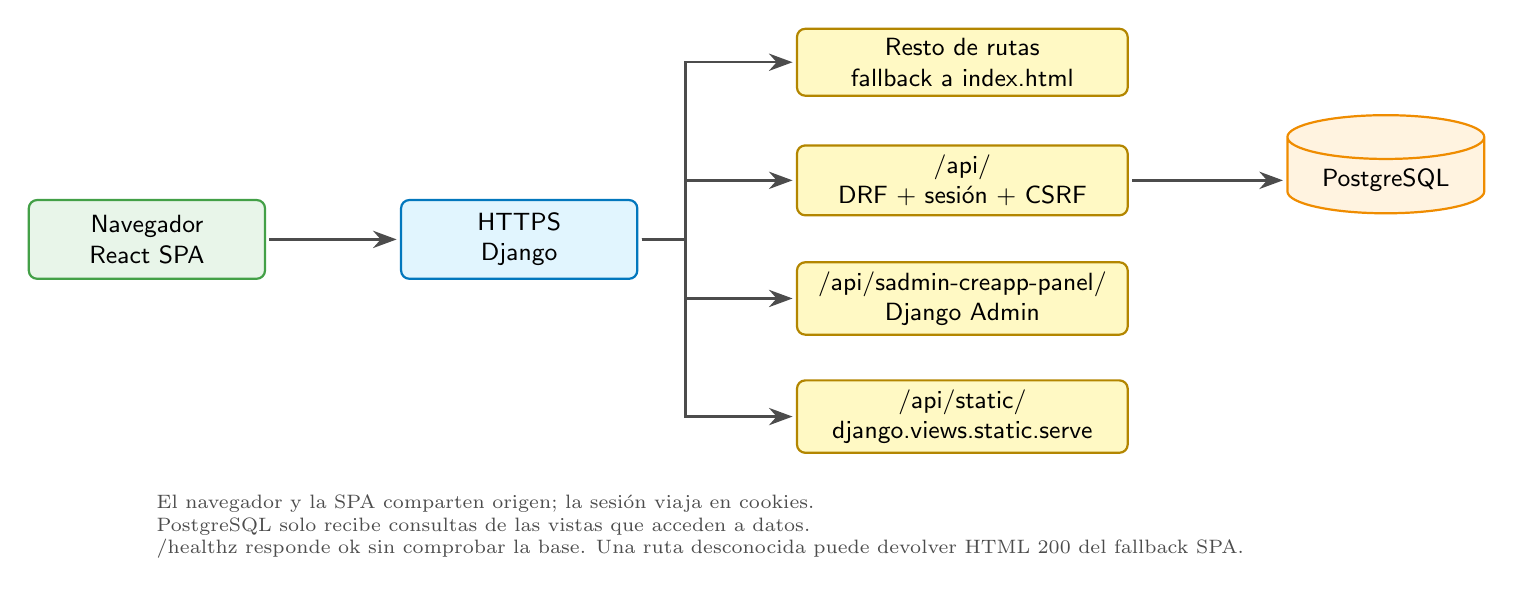
\begin{tikzpicture}[
  font=\sffamily\small,>={Stealth[length=3mm,width=2.2mm]},
  client/.style={rectangle,rounded corners=3pt,draw=greenStroke,thick,fill=greenFill,minimum width=3.0cm,minimum height=1.0cm,align=center},
  app/.style={rectangle,rounded corners=3pt,draw=coreStroke,thick,fill=coreFill,minimum width=3.0cm,minimum height=1.0cm,align=center},
  route/.style={rectangle,rounded corners=3pt,draw=procStroke,thick,fill=procFill,minimum width=4.2cm,minimum height=0.85cm,align=center},
  db/.style={cylinder,draw=memStroke,thick,aspect=0.3,shape border rotate=90,fill=memFill,minimum width=2.5cm,minimum height=1.2cm,align=center},
  edge/.style={->,line width=.9pt,draw=black!70,shorten >=1.2pt,shorten <=1.2pt}
]
% Left-to-right request flow; each route has its own row to keep labels clear.
\node[client] (browser) at (0,0) {Navegador\\React SPA};
\node[app,right=1.7cm of browser] (django) {HTTPS\\Django};
\node[route,right=2.0cm of django,yshift=2.25cm] (spa) {Resto de rutas\\fallback a index.html};
\node[route,right=2.0cm of django,yshift=0.75cm] (api) {/api/\\DRF + sesión + CSRF};
\node[route,right=2.0cm of django,yshift=-0.75cm] (admin) {/api/sadmin-creapp-panel/\\Django Admin};
\node[route,right=2.0cm of django,yshift=-2.25cm] (static) {/api/static/\\django.views.static.serve};
\node[db,right=2.0cm of api] (postgres) {PostgreSQL};
\draw[edge] (browser) -- (django);
\draw[edge] (django.east) -- ++(0.6,0) |- (spa.west);
\draw[edge] (django.east) -- ++(0.6,0) |- (api.west);
\draw[edge] (django.east) -- ++(0.6,0) |- (admin.west);
\draw[edge] (django.east) -- ++(0.6,0) |- (static.west);
\draw[edge] (api.east) -- (postgres.west);
\node[font=\scriptsize,text=black!70,align=left,anchor=west] at (0,-3.65)
 {El navegador y la SPA comparten origen; la sesión viaja en cookies.\\
  PostgreSQL solo recibe consultas de las vistas que acceden a datos.\\
  /healthz responde ok sin comprobar la base. Una ruta desconocida puede devolver HTML 200 del fallback SPA.};
\end{tikzpicture}
\end{document}
